\section{Suliman}

\begin{minipage}{0.5\textwidth}
\textbf{Name}: Suliman\\
\textbf{Function}: Wise woman, source of information for the protagonists

\subsection{Internal World}

\textbf{Age \& Gender}: 70-80, Female \\
\textbf{Values \& Virtues}: Loyal to the king \\
\textbf{Personality}: Strong, compassionate\\
\textbf{Interests}: Magic \\
\textbf{Ethnic Group}: Human, Witch

\subsection{External World}
\textbf{Environment}: Wastelands, Castle of Kingsbury \\
\textbf{Education}: High-education \\
\textbf{Social \& Cultural Background}: She is the court magician of Ingary \\
\textbf{Look \& Feel}: Always elegantly dressed, even if she looks like an old woman she is still incredibly powerful and smart \\
\textbf{Job \& Experience}: Court magician \\

\end{minipage}%
%
\hfill\begin{minipage}{0.4\textwidth}
  \begin{figure}[H]
  
\includegraphics{Images/Characters/suliman}
  \caption{Suliman, movie version}
\end{figure}
\end{minipage}

% \begin{figure}[H]
 % 
\includegraphics{Images/Characters/suliman}
 % \caption{Suliman, movie version}
% \end{figure}

% \textbf{Name}: Suliman\\
% \textbf{Function}: Wise woman, source of information for the protagonists

% \subsection{Internal World}

% \textbf{Age \& Gender}: 70-80, Female \\
% \textbf{Values \& Virtues}: Loyal to the king \\
% \textbf{Personality}: Strong, compassionate\\
% \textbf{Interests}: Magic \\
% \textbf{Ethnic Group}: Human, Witch

% \subsection{External World}
% \textbf{Environment}: Wastelands, Castle of Ingary \\
% \textbf{Education}: High-education \\
% \textbf{Social \& Cultural Background}: She became part of the royal family \\
% \textbf{Look \& Feel}: Always elegantly dressed, even if she looks like an old woman she is still incredibly powerful and smart \\
% \textbf{Job \& Experience}: Royal witch\\

\subsubsection*{Relationships}
\begin{enumerate}
\item \textbf{Sophie}: She appreciates her determination, her strength and his will to help Howl and so she is glad to help her.
\item \textbf{Howl}: She thinks Howl is the best among her apprentices, so she respects and she is fond of him but she doesn't really  fear him.
\item \textbf{Calcifer}: She respects him due to the fact that he is a fire demon.
\item \textbf{Justin}: She feels emphatic for his unlucky situation.
\item \textbf{Mizar}: She barely knows her because Mizar were the former court magician of Ingary, but she never met her.
\item \textbf{Belzel}: She is only aware of stories that tell about a djinn who lives in the desert in the south of Ingary, but she doesn't even know his name.
\end{enumerate}

\begin{figure}[H]
  \centering
  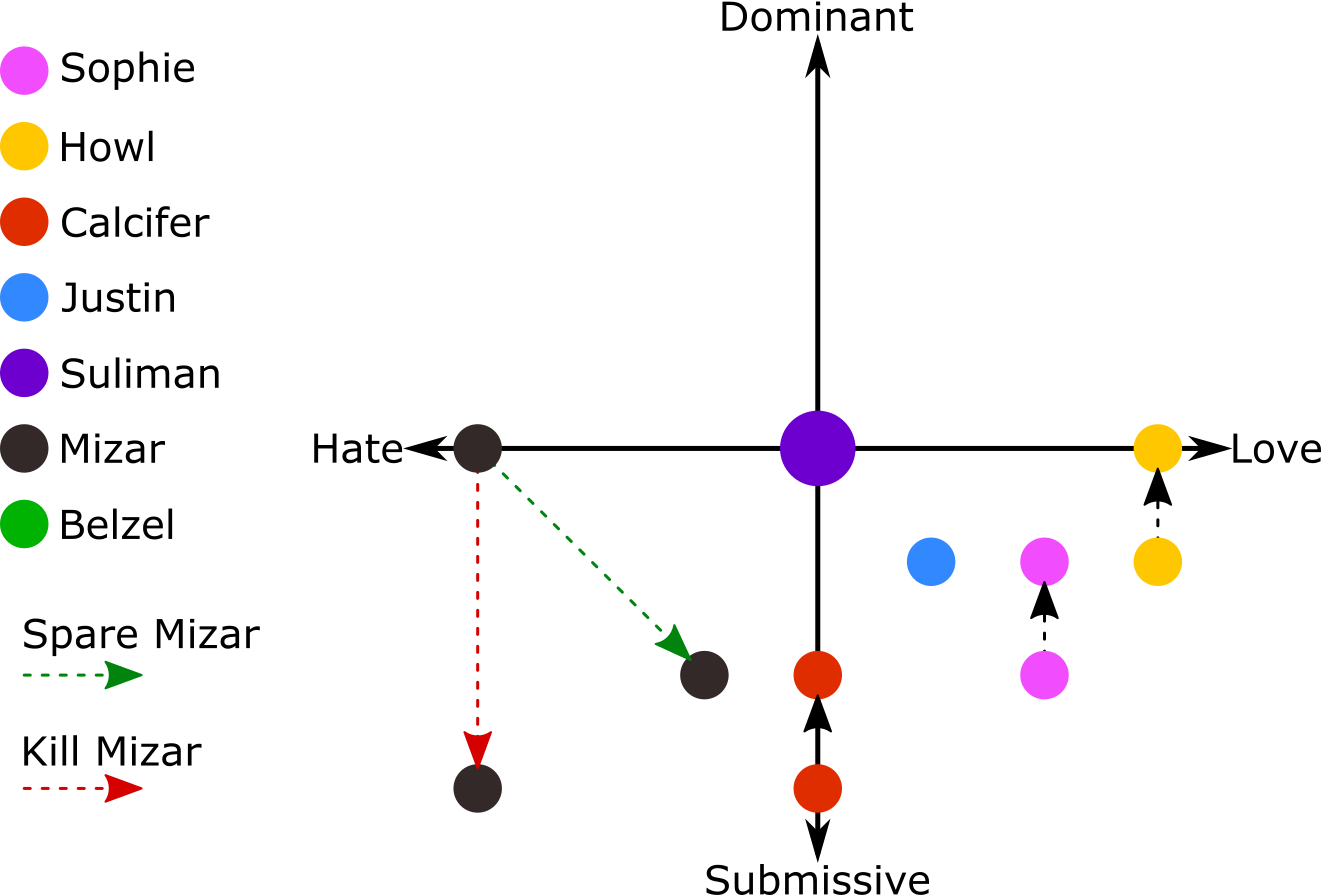
\includegraphics[width=8cm]{Images/SVG/Exported/Circumplexes/sulimanCircumplex}
  \caption{Circumplex of Suliman}
\end{figure}

\begin{figure}[H]
  \centering
   
\includegraphics[width=8cm]{Images/SVG/Exported/Evolutions/sulimanEvolution}
  \caption{Evolutions of Suliman}
\end{figure}

\subsection{Description}
She is an old woman but she is still feared by everyone because she is one of the most powerful witch in the whole kingdom. She is an able politician and leader, but she also cares for people's problems and she do whatever she can to help them.

\subsection{Background story}
She has been well educated in a noble family and she studied magic for several years.

She became court magician of Ingary after Mizar has left.

She has been Howl’s teacher.
